\documentclass{beamer}
\usepackage{tikz}
\usepackage{nicematrix}
\usepackage{amsmath}
\usepackage{empheq}
\usepackage{mathtools}
\usetheme{Madrid} % You can change the theme to your preference



\title{Statistiques pour données de comptage}
\author{Bastien Batardière}
\institute{INRAe}
\date{\today}

\begin{document}

\newcommand{\tikzmark}[1]{\tikz[overlay, remember picture] \coordinate (#1);}

\begin{frame}
  \titlepage
\end{frame}

\begin{frame}
    \frametitle{Données de comptage}
    \centering
     \[
  \boldsymbol{Y} =  \bordermatrix{~  & \tikzmark{harrowleft}  &  &  &
                        & \tikzmark{harrowright}  \cr
                    \tikzmark{varrowtop}  & 12  & 0 & \cdots & 0 &  9  \cr
                     & 2 & 0 & \cdots & 0 & 0  \cr
                     & \vdots &  &  &  & \vdots  \cr
                 \tikzmark{varrowbottom}    & 341 & 5 & \cdots & 1 & 0  \cr
                    }
\]
\tikz[overlay,remember picture] {
  \draw[->] ([yshift=1ex]harrowleft) -- ([yshift=1ex]harrowright)
            node[midway,above] {variables};
  \draw[->] ([yshift=1.5ex,xshift=25ex]varrowtop) -- ([xshift=25ex]varrowbottom)
            node[near end,right] {individus};
}
\end{frame}



% \begin{frame}
%   \[
%   \begin{empheq}[right=\empheqrbrace]{align*}
%     \onslide<1->{\text{Covariance} & \quad Z_i \sim \mathcal{N}(\mu, \Sigma) \\}
%     \onslide<2->{\text{Séries temporelles} & \quad Z_i \sim \mathcal{N}(A Z_{i-1}, \Sigma) \\}
%     \onslide<3->{\text{Clustering} & \quad Z_i \sim \sum_{k=1}^K \alpha_k \mathcal{N}(\mu_k, \Sigma_k)}
%   \end{empheq}
%   \onslide<4->{\quad \Rightarrow \quad Y \sim \mathcal{P}(\exp(Z_i))}
%   \]
% \end{frame}
\begin{frame}
  \frametitle{Adaptation des tâches statistiques: PLN}
\[
\left.
\begin{array}{ll}
    \onslide<2->{\text{Covariance} & \quad Z_i \sim \mathcal{N}(\mu, \Sigma) \\} \\
    \onslide<3->{\text{Séries temporelles} & \quad Z_i \sim \mathcal{N}(A Z_{i-1}, \Sigma) \\} \\
    \onslide<4->{\text{Clustering} & \quad Z_i \sim \sum_{k=1}^K \alpha_k \mathcal{N}(\mu_k, \Sigma_k)} \\
\end{array}
\right\}
\onslide<1->{Y_i \sim \mathcal P(\exp(Z_i))}
\]
\end{frame}


\begin{frame}
    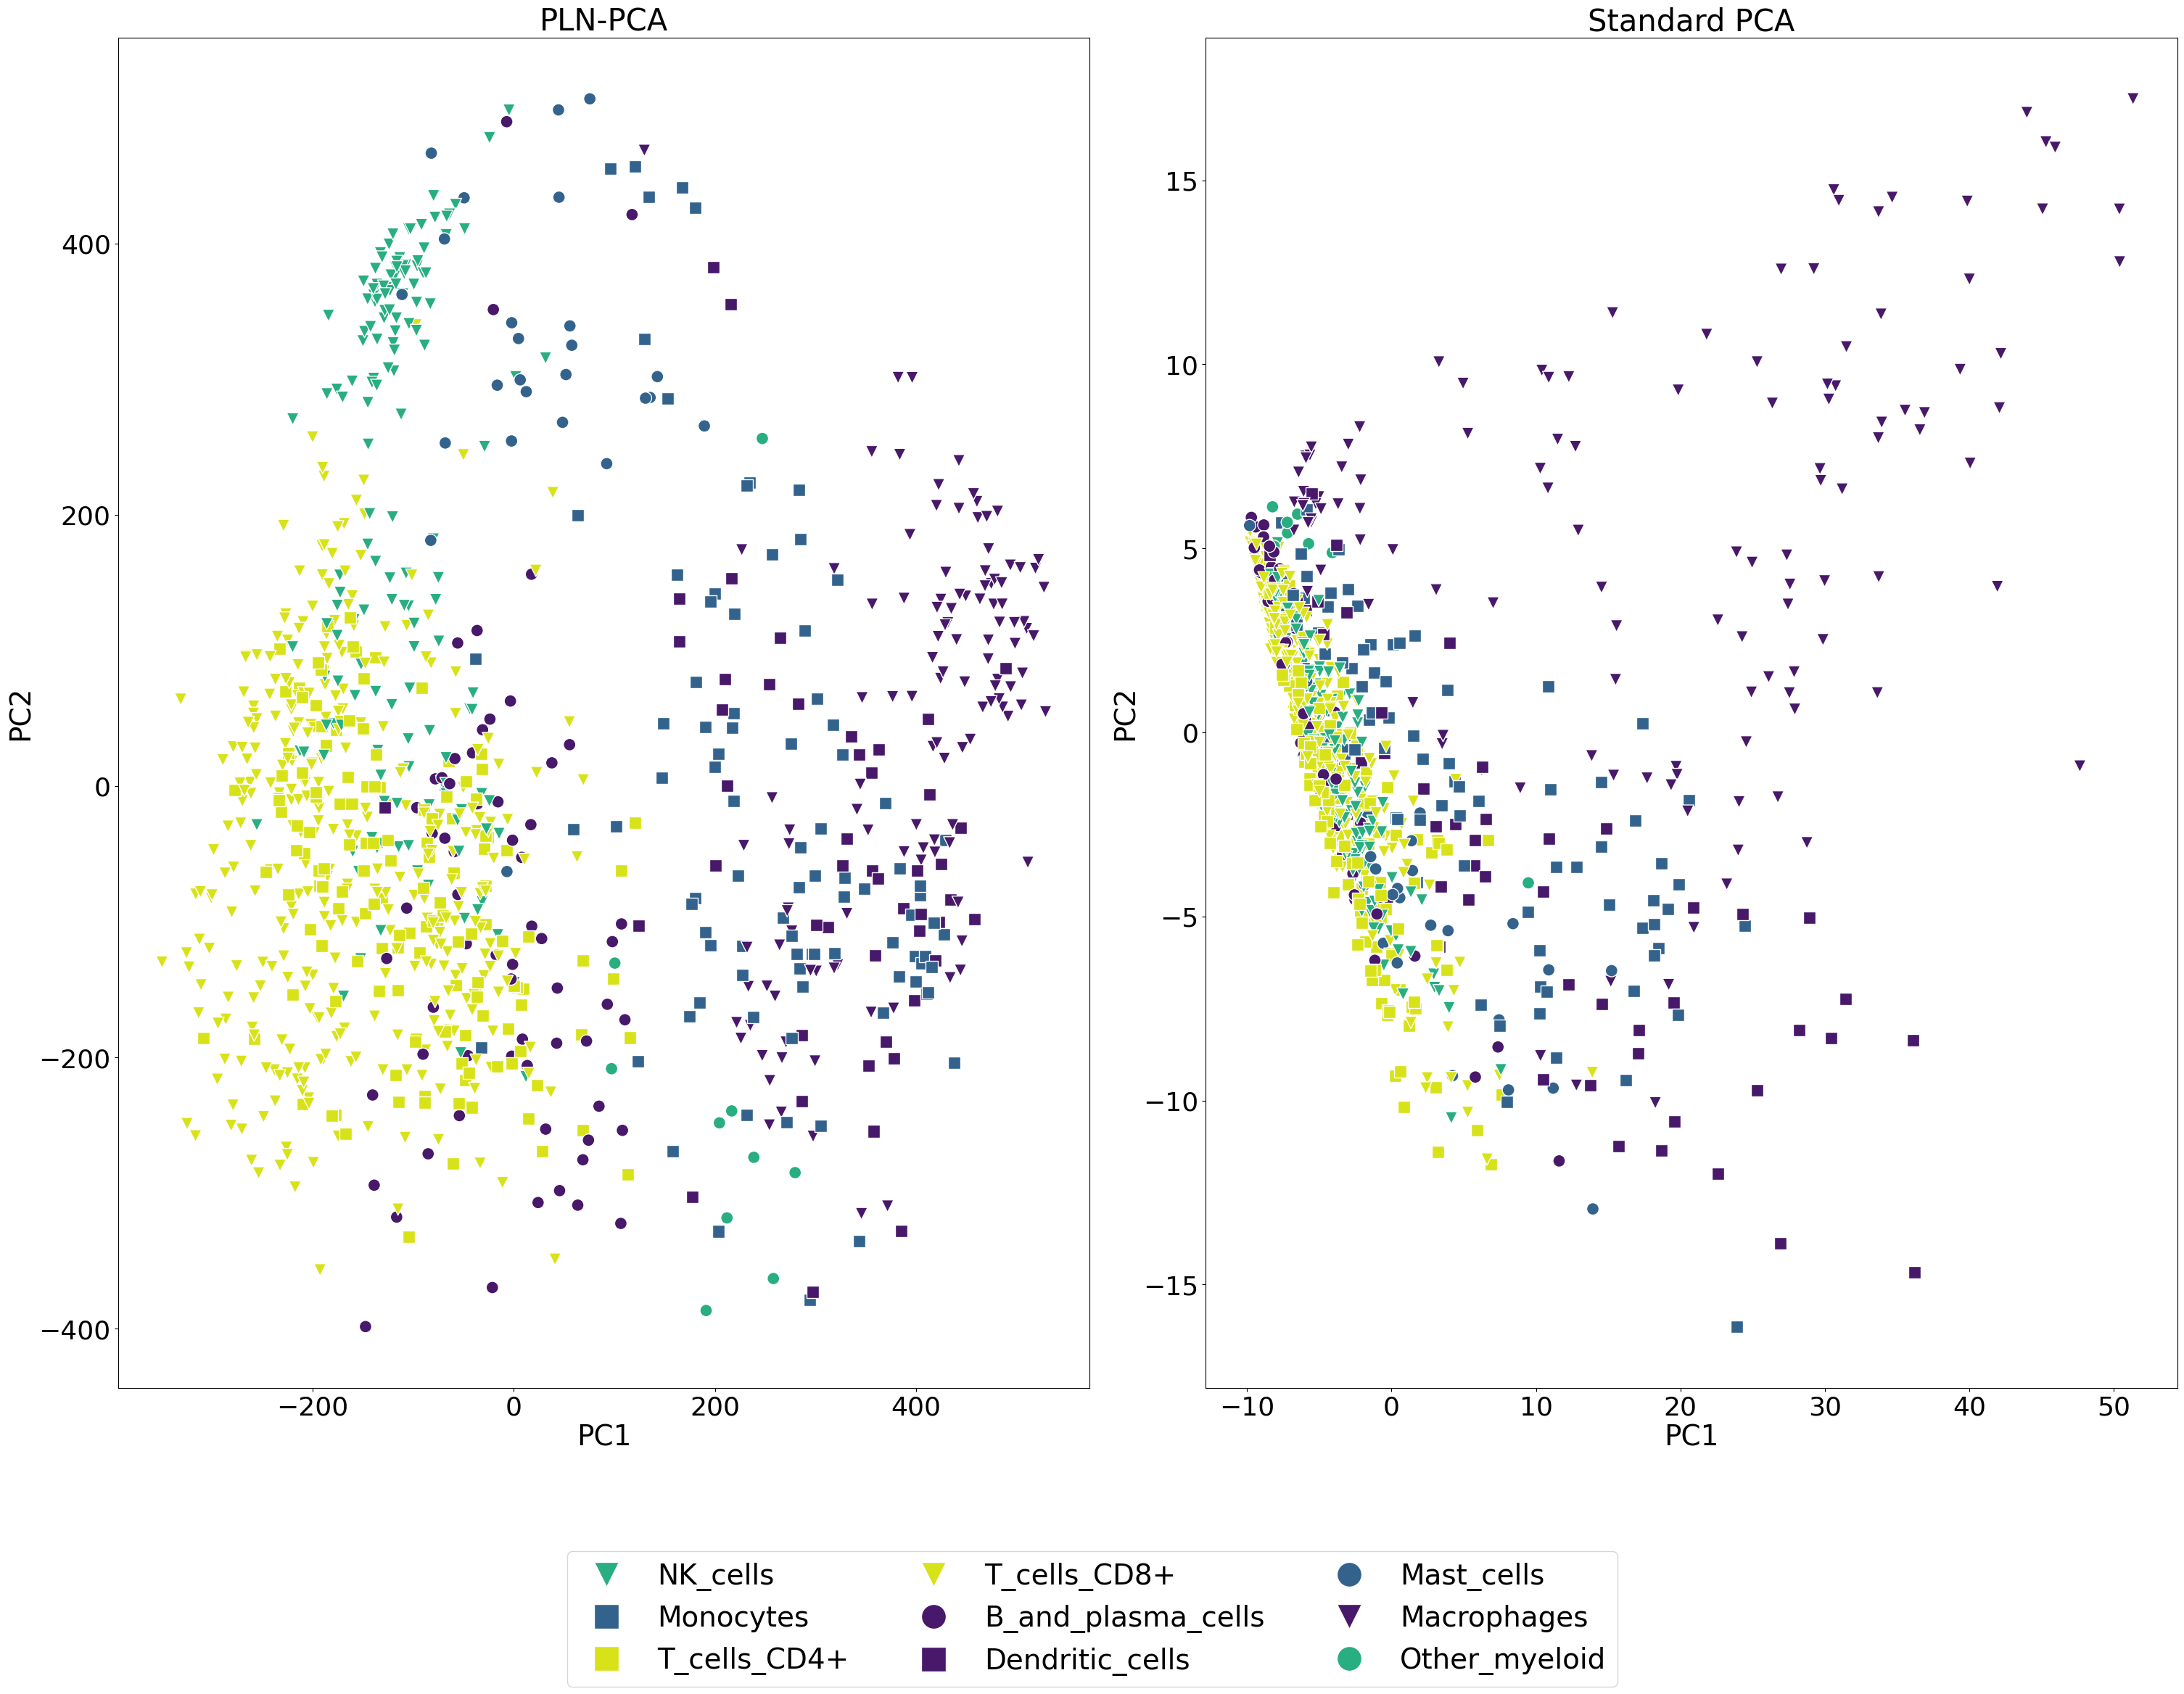
\includegraphics[width = \linewidth]{figures/plnpca_vs_pca_last.png}
\end{frame}



\begin{frame}
     \centering \Huge \texttt{pip install pyPLNmodels}

\end{frame}


\end{document}
